\section{Interaktion med sociale robotter}
\label{InteraktionSocialeRobotter}
%
Inden der dykkes ned i hvilke parametre, der har indflydelse på hvordan interaktionen med sociale robotter perciperes og accepteres, vil nogle mere generelle tendenser blive diskuteret. Det dækker blandt andet over køns-, alders- samt kulturelleforskelle i henhold til synet på sociale robotter. Dernæst gives der nogle eksempler på, hvordan relaterede studier har målt brugerens perception og accept af sociale robotter.
%
\subsection{Generelle tendenser}
\label{InteraktionSocialeRobotterGenerelleTendenser}
%
I den vestlige verden er vi i langt mindre grad villige til at acceptere sociale robotter end hvad der eksempelvis er tilfældet i Japan, \parencite[s. 28]{PDF:InTheCompanyofRobots}. Det skyldes, ifølge \textcite[s. 28]{PDF:InTheCompanyofRobots}, at der er en indgroede frygt for maskiner og følelsen af manglende kontrol, hvilket ikke er tilfældet i den Japanske kultur, som åndeliggøre robotter. At mennesker i den vestlige verden frygter robotter kan, blandt andet, retfærdiggøres med at i 2012 angav 87 \% af borgerne i Europa at de aldrig har været i kontakt med en robot, hverken i hjemmet eller på ens arbejdsplads, \parencite[s. 40]{PDF:PerceptionAcceptance}. I en undersøgelse, beskrevet af \textcite[s. 41]{PDF:PerceptionAcceptance}, fremgår det at synet på robotter ikke har ændret sig de sidste 35 år. Når robotterne, ved brug af tegninger, visualiseres så minder de i høj grad om robottypen: \textit{Non assistive robots}, illustreret på \autoref{fig:CategorizationOfRobots}. Endvidere tyder det på, at Europærer frygter, at de vil miste deres job til robotten og at robotten er til for at erstatte mennesket, \parencite[s. 22]{PDF:RobotShiftFromIPtoSR}.   

Derudover er der en tendens til, at mænd i højere grad perciperer robotten som menneskeagtig sammenlignet med kvinder, som i langt højere grad perciperer robotten som en maskine, \parencite[s. 28]{PDF:InTheCompanyofRobots}. Ifølge \textcite[s. 1479]{PDF:ExploringInfluencingVariable}, perciperer mænd robotter som værende mere brugbare, de har større intention om at bruge dem og de er mere villige til at acceptere robotter end kvinder er.  

Ydermere argumenterer \textcite[s. 2]{PDF:SharingALifeHarvey} for, at den ældre population i højere grad accepterer sociale robotter, sammenlignet med den yngre population. Det antages, at en af årsagerne til det formentlig skyldes, at der anvendes sociale robotter i ældreplejen eksempelvis til mindske følelsen af ensomhed, \fullref{EksisterendeSocialeRobotter}. I mere praktiske situation, som eksempelvis rengøring, tøjvask og lignende, foretrækker ældre robotter fremfor mennesker, hvorimod hvis opgaverne er omsorgsrelateret foretrækkes mennesker, \parencite[s. 22]{PDF:RobotShiftFromIPtoSR}.

\subsection{Parametre, der har indflydelse på accept og interaktion med sociale robotter}
\label{InteraktionSocialeRobotterParametre}
%
Der er to overordene kategorier af parametre: \textit{Utilitarian} og \textit{Hedonic}, først nævnte dækker over det praktiske og anvendelige aspekt ved at interagere med en social robot, hvor sidst nævnte relateres til brugerens oplevelse af at anvende den sociale robot, \textcite[s. 1476]{PDF:SharingALifeHarvey}. Da disse parametre har indflydelse på hvorvidt brugeren udfører en bestem adfærd, skal der tages højde for følgende:\blankline
%
\begin{quotation}
\textit{
  \begin{enumerate}
  \item the likely positive or negative consequences of the behavior
  \item the approval or disapproval of the behavior by respected individuals or groups, and
  \item the factors that may facilitate or impede performance of the behavior.
\end{enumerate}}
\textcite[s. 1477]{PDF:SharingALifeHarvey}\blankline
\end{quotation}
\noindent
%
Anvendes de tre overvejelser til at undersøge brugerens accept afspejler de, ifølge \textcite[s. 1477]{PDF:SharingALifeHarvey}, henholdvist brugerens evaluering af robotten, hvilke sociale normative overbevisninger der tilskrives robotten ved brug samt hvilke kontekstuelle faktorer der spiller ind ved brug.

\subsubsection*{Utilitarian}
\label{InteraktionSocialeRobotterParametreUtilitarian}
%
Som nævnt dækker \textit{utilitarian} parametre over det praktiske og anvendelige aspekt ved at interagere med en social robot. I følgende afsnit belyses hvilke parametre der har indflydelse på det praktiske såvel som det anvendelige aspekt. Der tages primært udgangspunkt i \textcite[s. 1477]{PDF:SharingALifeHarvey}.
%
\begin{figure}[H]
\centering
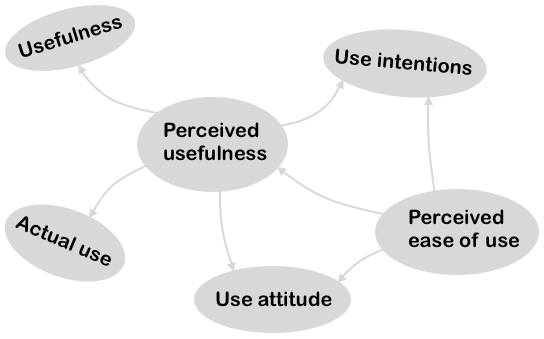
\includegraphics[width = 0.75\textwidth]{Figure/UtilitarianParameters} 
\caption{Sammenhængen mellem de seks forskellige parametre, der har indflydelse på det praktiske og anvendelige aspekt. Pilene indikerer hvilken retning indflydelsen er mellem to parametre.}
\label{fig:UtilitarianParameters}
\end{figure}
\noindent 
%
Baseret på \textcite[s. 1477]{PDF:SharingALifeHarvey} defineres \textit{usefulness} som værende brugerens overbevisning om, at robotten vil forbedre de daglige aktiviteter. Ifølge \textcite[s. 11]{PDF:SharingALifeHarvey} tyder det på, at \textit{usefulness} er en vigtig parametre, der kan bidrage til langtidssigtet forhold mellem bruger og robot. \textit{Ease of use} defineres som værende brugerens overbevisning om, at det nemt at anvende robotten. Derudover argumenterer \textcite[s. 1477]{PDF:SharingALifeHarvey} for, at i situationer hvor robotten skal indgå i en social interaktion med mennesker, er det nødvendigt at robotten gengiver menneskeagtige træk for, at brugeren føler sig komfortabel nok til at indgå i interaktionen. Robottens evne til at tilpasse sig den sociale kontekst afhængigt af brugeres behov, defineres som \textit{perceived adaptability}. Ifølge \textcite[s. 1477]{PDF:SharingALifeHarvey}, har \textit{perceived adaptability} indflydelse på \textit{perceived usefulness}, \textit{use attitude}, \textit{use intentions}, som er repræsenteret på \autoref{fig:UtilitarianParameters}. Derudover har \textit{perceived adaptability} indflydelse på \textit{enjoyment}. Ydermere tyder det på at \textit{intelligence}, har en effekt på hvor realistiske robotten perciperes, \parencite[s. 1477]{PDF:ExploringInfluencingVariable}.   
%
\subsubsection*{Hedonic}
\label{InteraktionSocialeRobotterParametreHedonic}
%
Som nævnt dækker \textit{hedonic} parametre over brugerens oplevelse af at anvende den sociale robot. I følgende afsnit belyses hvilke parametre der har indflydelse på det dette. Der tages primært udgangspunkt i \textcite[ss. 1477-1478]{PDF:SharingALifeHarvey}.
%
\begin{figure}[H]
\centering
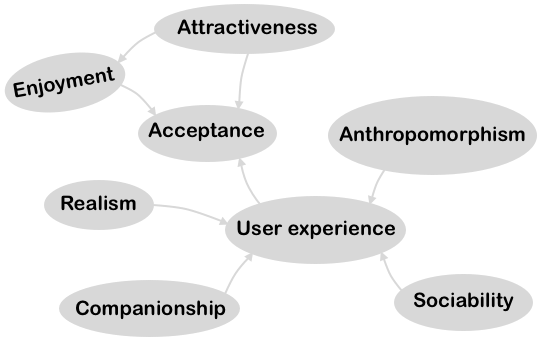
\includegraphics[width = 0.75\textwidth]{Figure/HedonicParameters} 
\caption{Sammenhængen mellem de otte forskellige parametre, der har indflydelse på brugerens oplevelse. Pilene indikerer hvilken retning indflydelsen er mellem to parametre.}
\label{fig:HedonicParameters}
\end{figure}
\noindent 
%
Baseret på \textcite[s. 1477]{PDF:ExploringInfluencingVariable} har både \textit{enjoyment}, der defineres som værende følelsen af fornøjelse eller glæde forbundet med brug, og \textit{attractiveness}, der defineres som værende den positive evaluering af robottens udseende, på flere af de parametre gengivet på \autoref{fig:UtilitarianParameters}. \textit{Enjoyment} har indflydelse på \textit{ease of use}, \textit{use attitude} samt \textit{use intentions}. Derimod har \textit{attractiveness} indflydelse på \textit{usefulness} og \textit{ease of use}.  




Together with these general variables of technology acceptance, for social robots specifically the variables of anthropomorphism, realism, sociability and companionship also influence the user experience with these robots. SIDE 1477
  
  
 This phenomenon is known as anthropomorphism. Anthropomorphism is a tendency to regard and describe object in human terms, attributing human characteristics to them with the intention to rationalize their actions [36]. As people feel the need to control their environment, those who feel uncertain are more likely to anthropomorphize a social robot as it helps then to ex- plain, control and predict the behavior of a nonhuman agent [37]. SIDE 1478
 
 Perceiving the presence of a social entity when using an interac- tive system has been found to be a crucial factor in the process of accepting these technologies [7,35,38], as it affects usefulness, attitude towards robots, social influence, companionship, use at- titude and use intention [7,16,18,38]. Being anthropomorphized, social robots could also be viewed as being genuine. Several stud- ies demonstrate that the increase of realism may indeed improve the human–robot interaction [32]. In the field of human–robot in- teraction, researchers have suggested that matching the realism of robot appearance and behavior can improve interactions with hu- mans. Human-likeness of a robot’s appearance is preferred when it is a counterpart to the sociability of their behavior [21]. The realism of the robot is defined as the degree to which users be- lieve the robot behaves and responds realistically, and research demonstrates that realism may improve the human–robot interac- tion [25]. Moreover, more realistic robotic interfaces are perceived as more intelligent [39]. People across gender, age and culture tend to perceive a robot who possesses a lifelike appearance as a friendly companion [40]. SIDE 1478
 
 As social robots are designed for the social inter- action, they should possess a considerable amount of social skills. In observing human–human interactions, there are several charac- teristics that make certain people more likeable than others in so- cial interactions. These characteristics are conceptually combined as social competence [41] or sociability. Adapted to robotics, so- ciability is defined as the users’ belief that the robot possesses the social, emotional, and cognitive skills required for successful social adaptation. The sociability of a robot also affects its usefulness and people’s attitude towards use SIDE 1478
 
 n fu- turistic social roles of robots, 70\% of the participants have indi- cated that they would eventually prefer to have companionship with robots. Companionship is defined as the user’s perceived pos- sibility to build a relationship with the robot [38]. Bonding with a social robot influences the intention to continuing its use [6,43,44]. SIDE 1478










Kom ind på de forskellige parametre der har indflydelse på brugerens oplevelse af hvordan det er at interagere med robotten. F.eks. online community (folk der spiller online spil hvor der er en form for kommunikation mellem én eller flere avatars) \blankline
%
Brug Harvey, det japanske studie hvor de tester to robotter i et supermarket, brug exploring influencing variables (Kan være en idé at lave en figur som vise hvordan de hænger sammen - f.eks. den "brainstorm" jeg har lavet på papir), how social distance shapes human-robot interaction og andre. \blankline
%
%
Brug det her argument til at forsvare hvorfor det også er vigtigt at undersøge hedonic variabels og hvilken indflydelse de har: Airports were regarded as purely utilitarian infrastructures in the past. To mitigate negative experiences with prolonged security protocols, airports have used rebranding strategies to integrate their surroundings or to become reinvented as destinations in their own right instead of just thoroughfares (Tsui, 2014). Aside from operational quality assurance, destination-focused rebranding emphasizes the need to create enjoyable experiences at airports \textcite[s. 352]{PDF:TheImpactOfTraveler}.\blankline
%
Out of the five widely used personality dimensions, namely the extroversion, agreeableness, conscientiousness, neuroticism, and openness [5], the most important dimensions for social interactions are those that concern individual differences in social behavior, namely extroversion and agreeableness or their common rotations, ‘friendliness’ and ‘dominance’ [6]. Fra Personality of social robots perceived trough the appearance side. 272.

\subsubsection{Bevægelsesmønstre og udseende}
\label{InteraktionSocialeRobotterParametreBevaegelsesmoenstre}
%


3 For example, many southern Europeans and Japanese have an intimate distance (reserved for close friends and family) of only 20-30cm compared to 46-122cm of the Americans and northern Europeans. Europeans might refer to Asians as ‘pushy’ and ‘familiar’ and Asians might refer to Europeans and Americans as ‘cold’ and ‘stand-offish’. There are also differences in rural vs. urban spatial zones. People raised in more rural, less populated areas need more personal space, than those raised in densely populated cities. side 178 \textcite[s. 178]{PDF:HowMayIServeYou}.

Most subjects stated that the robot moved too slowly or about right at 0.4m/s, while nobody rated that the robot moved too fast. This suggests that (especially after a longer habituation period), most subjects would prefer the robot to move at a faster speed. It would therefore be reasonable to set the default robot speed at a relatively slow 0.4m/s and then perhaps increase the approach speed over time or in response to the user’s wishes or preferences. \textcite[s. 178]{PDF:HowMayIServeYou}. 

The frontal approach was seen as uncomfortable, impractical, in some cases even threatening or confrontational, and should thus be avoided. This result is in line with human-human situations where standing or sitting at an angle of 45 degrees to each other can reduce feelings of aggression and confrontation \textcite[s. 178]{PDF:HowMayIServeYou}

From psychological studies [14] it has been found that women tend to stand slightly closer to one another, face each other more, and touch each other more, compared to men interacting with other men. \textcite[s. 178]{PDF:HowMayIServeYou}. 

\subsection{Hvordan kan oplevelsen måles?}
\label{InteraktionSocialeRobotterOplevelse}
%
Mange undersøgelser laves bare med spørgeskemaer, likert-skalaer, korte interaktioner med robotten, videoklip med robotten. 

Inddrag Personality of social robots perceived through the appearances.

Kom ind på hvordan det måles, hvad har andre gjort i forhold til det (overvej om det skal være en sektion for sig selv).\blankline












